%% 美赛模板:正文部分

\documentclass[12pt]{article}  % 官方要求字号不小于 12 号,此处选择 12 号字体

% 本模板不需要填写年份,以当前电脑时间自动生成
% 请在以下的方括号中填写队伍控制号
\usepackage[2332102]{easymcm}  % 载入 EasyMCM 模板文件
\problem{Y}  % 请在此处填写题号
%\usepackage{mathptmx}  % 这是 Times 字体,中规中矩 
%\usepackage{mathpazo}  % 这是 COMAP 官方杂志采用的更好看的 Palatino 字体,可替代以上的 mathptmx 宏包
\usepackage{newtxtext}
\newcommand{\upcite}[1]{\textsuperscript{\textsuperscript{\cite{#1}}}} 
\title{Title}  % 标题

% 如需要修改题头(默认为 MCM/ICM),请使用以下命令(此处修改为 MCM)
\renewcommand{\contest}{MCM}

% 文档开始
\begin{document}

% 此处填写摘要内容
\begin{abstract}
    Sailboats fulfill diverse roles, fueling a thriving secondary market. 
    Brokers, facing numerous complex factors, struggle to determine reasonable pricing. 
    A tool to assist in comprehensive evaluations and rational pricing for used boats is urgently needed.
    
    This paper aims to construct a reliable model based on existing datasets, 
    which can provide a reasonable explanation for the pricing of the second-hand sailboat market. 
    It also analyzes the impact of different factors and indicators on prices. 
    Finally, the model will be applied to the second-hand sailboat market in Hong Kong to provide a reasonable and accurate pricing rule.

    For Data Exploration, \dots

    For Problem(a), \dots

    For Problem(b), \dots

    For Problem(c), \dots

    For Problem(d), \dots

    For Problem(e), \dots

    At the very last, we analyze the strengths and weaknesses of our model as well as its
sensitivity, whose results show that our model has high robustness, precision and accuracy.
After that, a report is attached.




    % 美赛论文中无需注明关键字。若您一定要使用,
    % 请将以下两行的注释号 '%' 去除,以使其生效
    \vspace{5pt}
    \textbf{Keywords}:  Linear interpolation, Adaptive Density-Based Clustering, Heuristic Hierarchical Multiple Regression, Deep Forest Model,  Machine Learning, Analysis of Variance.
 

\end{abstract}

\maketitle  % 生成 Summary Sheet
\tableofcontents  % 生成目录


% 正文开始
\section{Introduction}
% 问题背景
\subsection{Background}
In our daily lives, sailboats are not only a means of transportation, but also serve as leisure and entertainment, and even for competitive sports. As a result, the growing demand for sailboats has given rise to a thriving boat market, which has gradually developed into a secondary market. In the secondary market, buyers and sellers usually trade through brokers, who play a crucial role in the transaction process.

For brokers, it is essential to be familiar with the used sailboat market, comprehensively consider various factors, and make reasonable pricing for the used sailboats in order to facilitate a successful transaction. However, the factors affecting the price of used sailboats are numerous and complex, with different brands, variants of boats, years, depreciation rates, as well as local consumption levels and geographical environments having significant impacts. The intertwined influences of these complex factors make it difficult to determine the pricing in the used sailboat market, and it is challenging to come up with a reasonable price that takes all factors into account.

Therefore, brokers urgently need a tool to assist them in making more reasonable and comprehensive evaluations of used sailboats, and to make the pricing in the used sailboat market more rational.
%问题重述
\subsection{Problem Restatement}
\textbf{Problem (a) :}
\begin{itemize}
    \item Develop a prediction model to explain the listing price of each of the sailboats in the provided spreadsheet.
    \item Discuss the precision of our estimate for each sailboat variant's price.
\end{itemize}

\textbf{Problem (b) :}
\begin{itemize}
    \item Determine whether region has an impact on the price of second-hand boats and explain the effect.
    \item Discuss whether any regional effect is consistent across all sailboat variants.
    \item Address the practical and statistical significance of any regional effects noted.
\end{itemize}

\textbf{Problem (c) :}
\begin{itemize}
    \item Based on the model, find out how it can be useful in the Hong Kong market.
    \item Choose one subset and model the regional effect of Hong Kong on each sailboat prices.
    \item Assess whether  the effect is the same for both catamarans and monohull sailboats.
\end{itemize}

\textbf{Problem (d) :}
\begin{itemize}
    \item Identify and discuss additional informative conclusions drawn from the data.
\end{itemize}

\textbf{Problem (e) :}
\begin{itemize}
    \item Create a one-to two-page report with well-chosen graphics to assist the Hong Kong sailboat broker to understand your findings.
\end{itemize}
%我们的工作
\subsection{Our work \& Model Overview}
\begin{figure}[htbp]
    \centering
    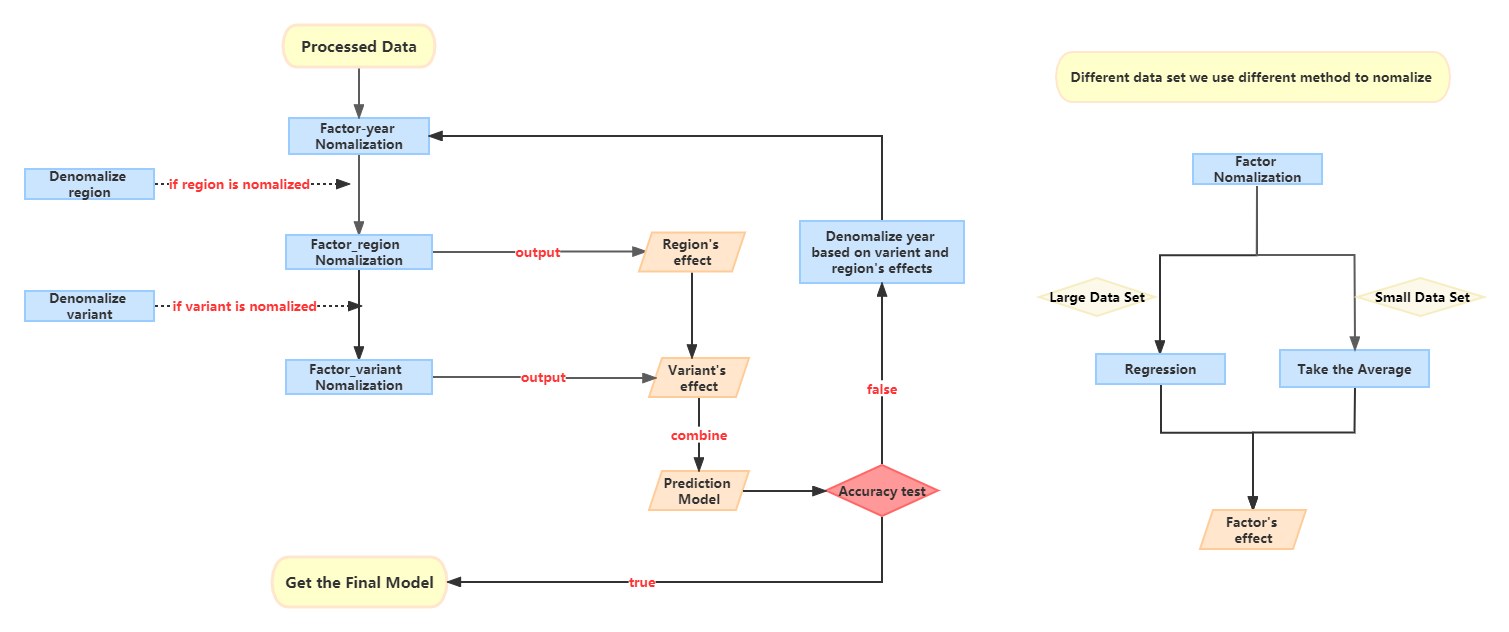
\includegraphics[width=1\textwidth]{OurWork.png}
    \caption{Model Framework}\label{fig:OurWork}
\end{figure}
Our team began by meticulously cleaning, expanding, and pre-analyzing the dataset using \textbf{Adaptive Density-Based Clustering} and \textbf{Linear interpolation} techniques. These methods allowed us to identify patterns and trends in the data, preparing it for subsequent modeling.

Next, we trained a \textbf{Heuristic Hierarchical Multiple Regression Model} to establish the relationship between year, region, variant, and price, and to abstract the effect of regions and variants on sailboat prices. This approach helped us capture the interactions between these variables and their influence on the pricing.

Following this, we employed a \textbf{Deep Forest Model} to train the relationship between region and variant factors and their respective effects. This advanced ensemble learning technique allowed us to predict the effect of unknown regions and variants, which in turn enabled us to further predict their prices.

As a result, we successfully developed a comprehensive and robust model (Figure \ref{fig:OurWork}) that is well-suited for Hong Kong brokers when pricing used sailboats. By leveraging the strengths of both Heuristic Hierarchical Multiple Regression and Deep Forest Models, our approach offers a reliable and accurate way to estimate the value of sailboats based on factors such as year, region, and variant. This model serves as a valuable tool for brokers and other stakeholders in the sailboat market, facilitating informed decision-making and ensuring fair pricing practices.

\section{Assumptions and Justifications}
% 问题假设
\subsection{Assumptions}
To simplify our problems, we make the following basic assumptions, each of which is
adequately justified.
\begin{itemize}
    \item The price of used sailboats is solely determined by the factors in the dataset.
    \item The factors in the dataset are independent and unrelated.
    \item The data in the dataset are all real, reasonable, and follow a certain pattern.
    \item For the used boats that need price prediction, we can obtain at least the same number of factors information as in the dataset.
    \item The pricing required by a broker should be reasonable and in accordance with market rules, rather than false pricing.
\end{itemize}
%符号含义
\subsection{Notations}
\ 
% 三线表示例
\begin{table}[!htbp]
\begin{center}
\begin{tabular}{cc}
	\toprule
	\multicolumn{1}{m{3cm}}{\centering Symbol}
	&\multicolumn{1}{m{8cm}}{\centering Definition}\\
	\midrule
	$l$ &Measurement data\\
	$L$ &Feature vector\\
	$F$ &The dimension of $L$\\
    $k$ &Search range\\
    $\lambda$ & The feature values of natural neighbors\\
    $nb_k(l)$ & The number of reverse neighbors of $l$ in the $k$-th iteration\\
    $R$ & Correlation coefficient\\
    $\hat{y}$ & The estimated value of $y$\\
    $\hat{\beta}$ & The estimated value of the regression coefficients\\
    $\textbf{X}, \textbf{Y}$ & The variables for which the correlation is to be tested \\
    $\textbf{P}$ & Measured value \\
    $\textbf{Q}$ & Simulated value \\ 
	\bottomrule
\end{tabular}
\end{center}
\end{table}
\section{Data Exploration}

\begin{figure}[htbp]
    \centering
    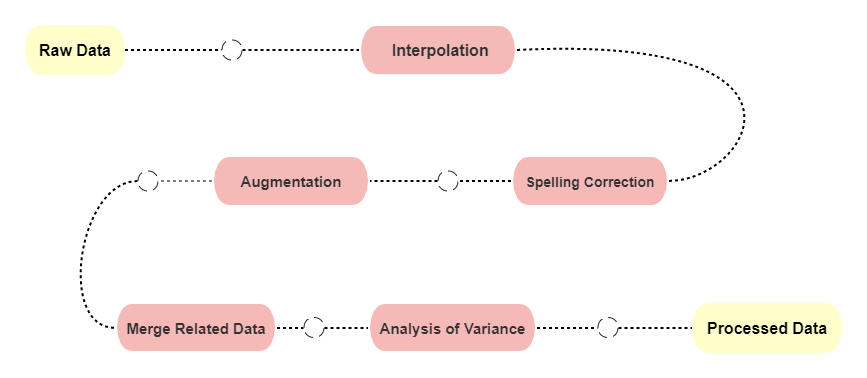
\includegraphics[width=.8\textwidth]{Data.png}
    \caption{Data Exploration}\label{fig:Data}
\end{figure}

\subsection{Data Cleaning}
First of all, we turn the \textbf{\texttt{xlsx}} format data sheet into \textbf{\texttt{csv}} format. 
The conversion causes some minor errors like extra spaces and unexcepted characters which can be easily filtered out by text editor and python string operating functions like \textbf{\texttt{strip()}} or so.

Secondly, we use \textbf{Linear interpolation} to fill in the missing data and then apply \textbf{Adaptive Density-Based Clustering} for spell correction,
resulting in a more complete and accurate dataset than the original.

Specificlly:

Based on the text-type variables, the feature matrix $L_i$ is used, and the Euclidean distance is used to calculate the text similarity:
$$dist(l_i,l_j)=\sqrt{\sum_{f=1}^{F}(L_i^f-L_j^f)^2}$$

Because ADC is a clustering iterative process, we first calculate the $k$-Nearest Neighbors:
$$NN_k(l_i)=\{l_j \in D|dist(l_i,l_j)\leq dist(l_i,o)\}$$

Then we define the Reverse Neighbors as:
$$RNN(l_i)=\{l_j \in D|l_i\in NN_k(l_j)\}$$

Applying $NN_k$ and $RNN(l)$ iteratively to obtain clustering centers, unclassified text samples are assigned to the nearest clustering center, and $\lambda$ is calculated as follows:
$$\lambda=min\{k|\sum_{i=1}^{n}f(nb_k(l_i))=0\quad or\quad \sum_{i=0}^{n}f(nb_k(l_i))=\sum_{i=0}^{n}f(nb_{k-1}(l_i))\}$$

Where $f(x)$ is defined as:
$$f(x)=
\begin{cases}
0,\quad otherwise\\1,\quad if\quad x=0
\end{cases}$$

Further more, we merge \textbf{Make} and \textbf{Variant} into a single feature, which we refer to as \textbf{Variant}.

Finally, we merge the corrected dataset with the accurate one after making necessary modifications.
\begin{figure}[htbp]
    \centering
    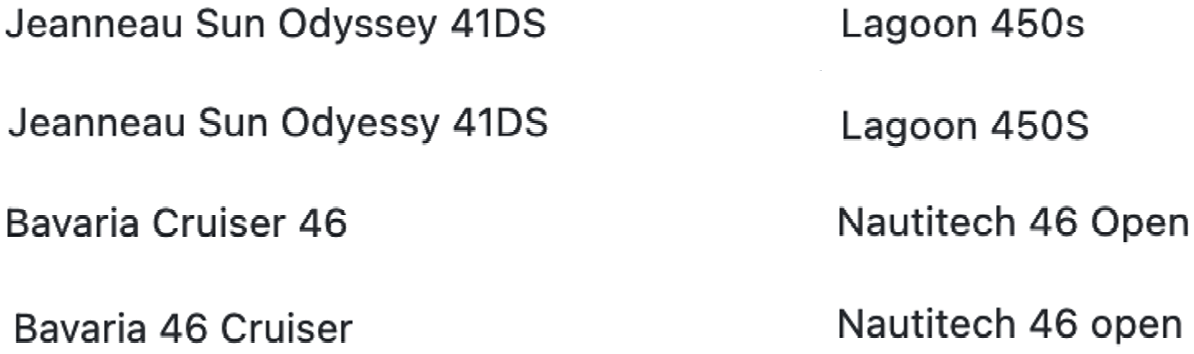
\includegraphics[width=0.7\textwidth]{error_data.png}
    \caption{Examples of error data}\label{fig:error_data}
\end{figure}

\subsection{Data Augmentation}

Our team diligently collected and organized additional ship attributes for the given dataset using Pandas' \texttt{read\_html} web scraping technique,
which allowed us to efficiently extract valuable information from various online sources. 
Simultaneously, we gathered the 2020 per capita GDP data of the relevant regions to provide important economic context that might influence sailboat prices.

Upon obtaining the data, we first employed Pandas' related functions to remove any duplicate entries, 
ensuring the dataset's integrity and uniqueness. 
Next, we addressed missing values by using linear interpolation, 
a technique that estimates missing data points by drawing upon the values of neighboring data points. 
This approach helped us create a more complete and reliable dataset for further analysis.

These data collection, organization, and preprocessing efforts significantly enriched the diversity of the data and expanded the dataset size.
By incorporating a wider range of sailboat features and relevant economic data, we were able to develop a more comprehensive understanding of the factors influencing sailboat prices. 
This extensive dataset laid a solid foundation for our subsequent modeling efforts, enabling us to create more accurate and reliable predictive models for sailboat pricing.

In conclusion, the meticulous data collection, organization, and preprocessing steps we undertook played a crucial role in the success of our modeling efforts. 
By addressing issues such as duplicates and missing values, and incorporating a diverse range of ship attributes and economic data,
we ensured the robustness and reliability of our dataset, paving the way for the development of highly effective predictive models.





\subsection{Data Analysis}
There is an abundance of labels related to sailboat specifications, which makes it challenging to discuss their individual influence on listing prices.
Attempting to directly perform regression on these labels using machine learning models can lead to \textbf{overfitting issues}, where the model becomes too specialized in fitting the training data and loses its ability to generalize well to new, unseen data.

Despite these challenges, we can still extract some relatively straightforward insights from the data, which can provide valuable theoretical support for our subsequent modeling efforts:
\begin{itemize}
    \item Time: Time is a quasi-continuous and ordered variable, exhibiting a clear linear relationship with the price of sailboats (as demonstrated in Figure \ref{fig:year_price} and Table \ref{table: correlation_coefficient}). As sailboats age, their value typically decreases, reflecting factors such as depreciation, wear and tear, and technological advancements in newer models.
    \item Variant and Region: These factors are undeniably related to sailboat prices; however, their unordered and non-continuous nature necessitates further analysis. Sailboat variants can encompass different designs, sizes, and features, which can significantly impact their value. Similarly, regional factors such as local demand, availability, economic conditions, and even cultural preferences can influence sailboat prices.
\end{itemize}
\begin{figure}[htbp]
    \centering
    \begin{subfigure}[b]{.4\textwidth}
    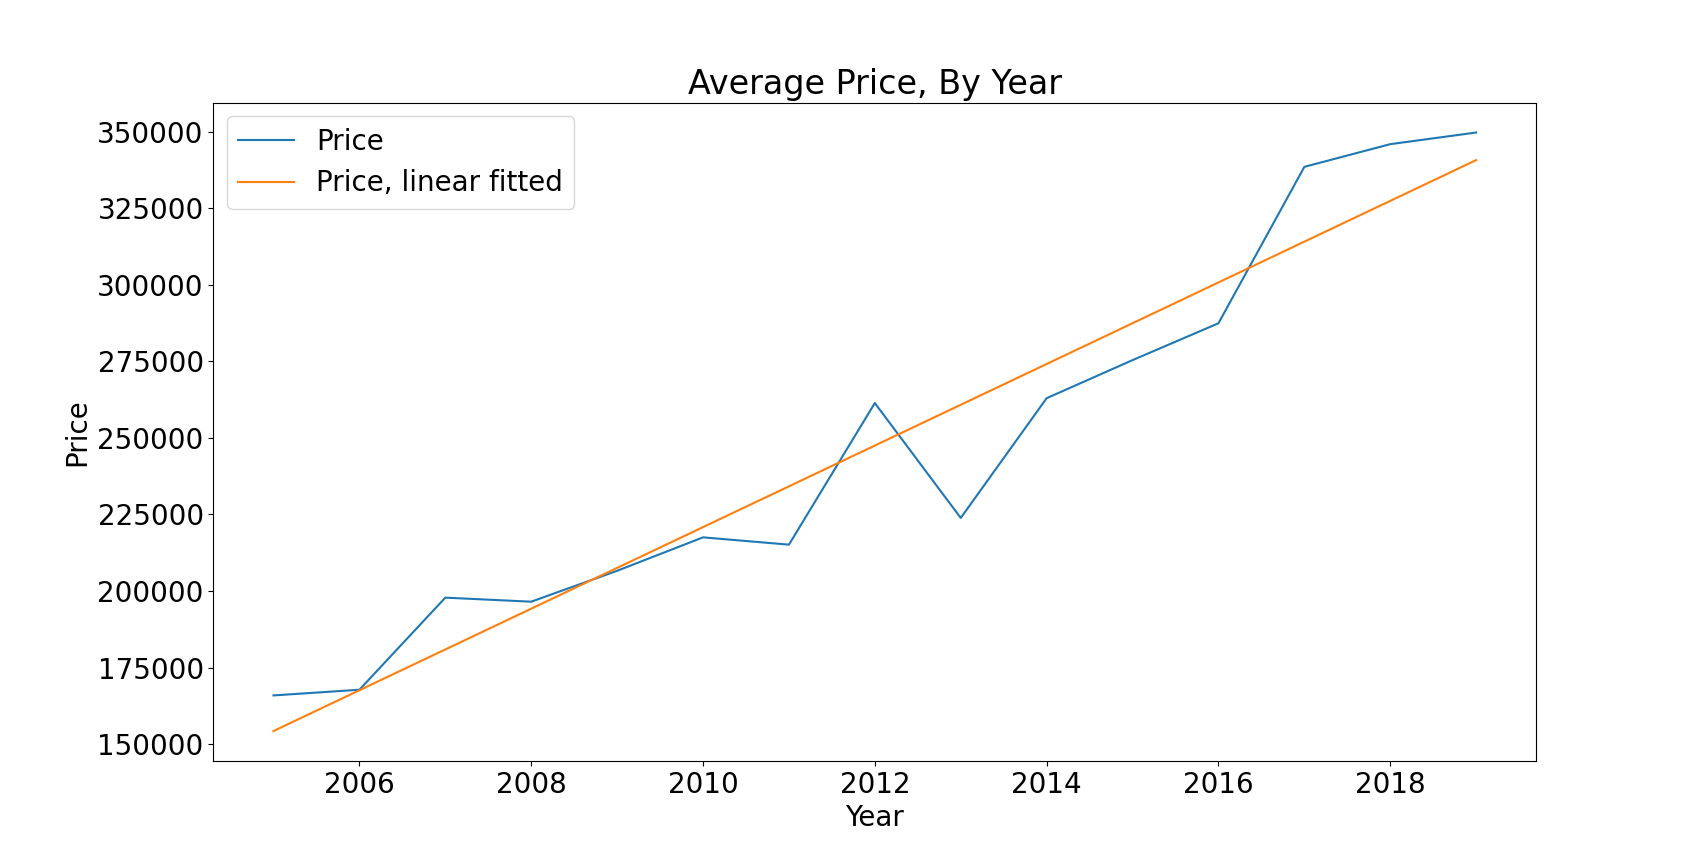
\includegraphics[width=\textwidth]{monohulled_price_year.png}
    \caption{Monohulled Sailboats}\label{subfig:mono_year}
    \end{subfigure}
    \begin{subfigure}[b]{.4\textwidth}
    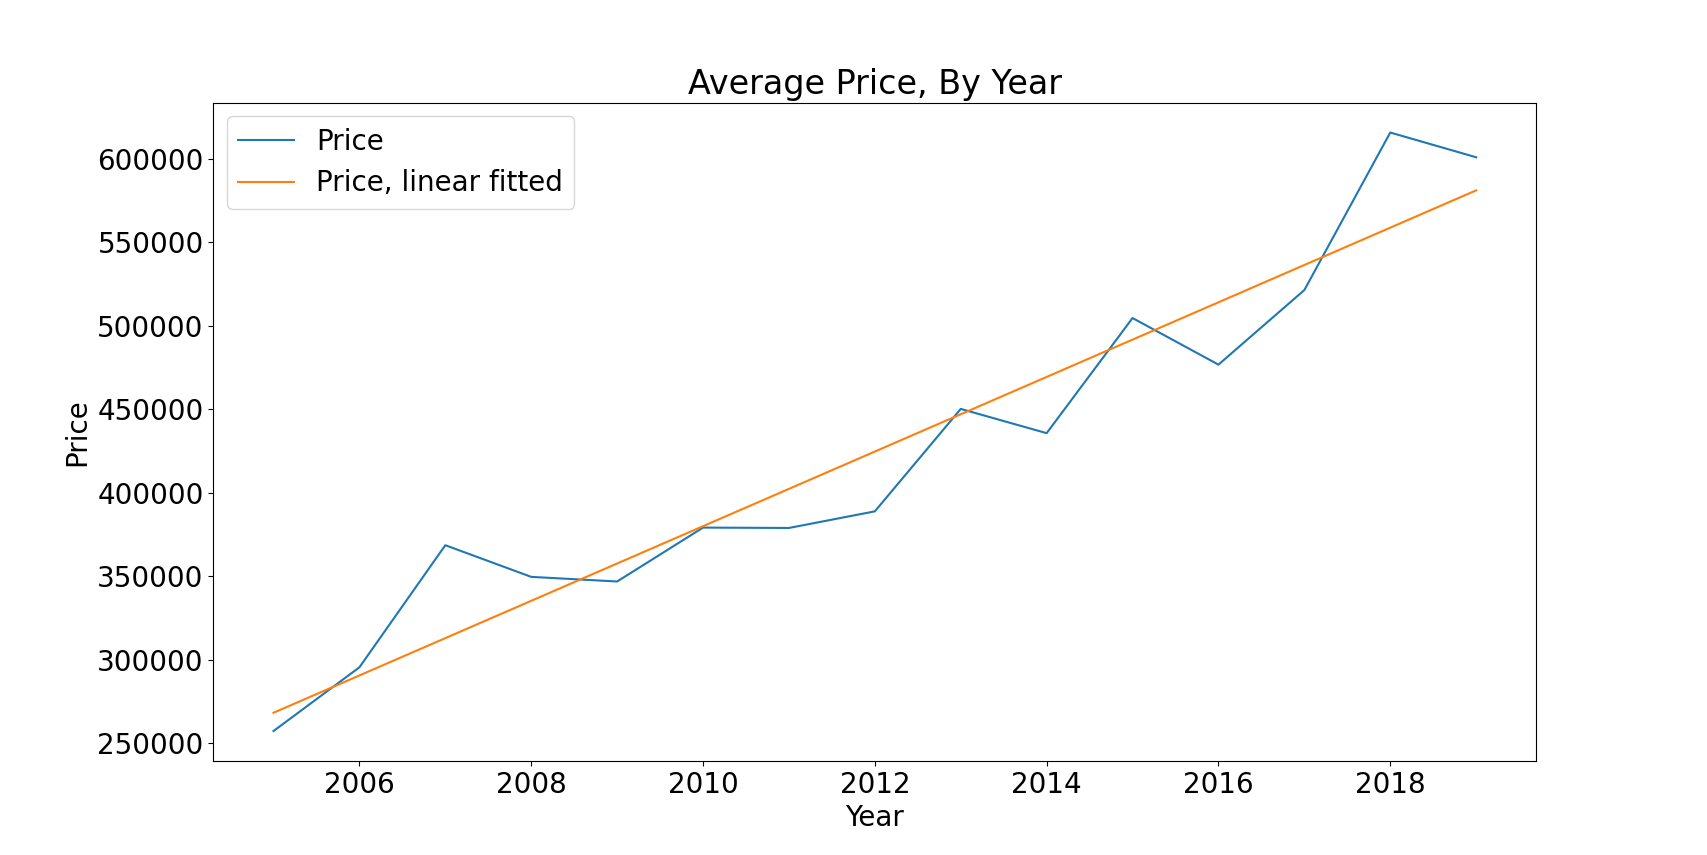
\includegraphics[width=\textwidth]{catamaran_price_year.png}
    \caption{Catamaran}\label{subfig:cata_year}
    \end{subfigure}
    \caption{The relationship between year and price}\label{fig:year_price}
\end{figure} 

\begin{table}[h!]
    \begin{center}
      \begin{tabular}{c|c|c|c}
        & Pearson & Spearman & Kendall\\
        \hline
        \hline
        Monohulled Sailboats&0.964 & 0.989 & 0.943 \\
        Catamaran  &0.960& 0.971 & 0.867\\
      \end{tabular}
      \caption{The correlation coefficient of year and price}\label{table: correlation_coefficient}
    \end{center}
\end{table}


\section{The Prediction Model of Used Sailboat Prices}

\subsection{The Establishment of The Model}
\subsubsection{Model 1 \textemdash  Heuristic Hierarchical Multiple Regression}

\emph{Model 1}, as illustrated in Figure \ref{fig:Model1}, is specifically designed to predict prices by taking into account input variables such as Year, Region, and Variant. To achieve accurate predictions, this model incorporates a heuristic hierarchical multiple regression approach, which distinguishes it from conventional regression methods. This innovative technique allows for a more nuanced understanding of the relationships between variables, ultimately leading to improved performance and reliability.

As for Hierarchical Multiple Regression, to solve the objective function for a given $n$ data points $(x_i, y_i)$:
$$L(y,f(x,w))=\sum_{i=1}^{n}[y_i-f(x_i,w_i)]^2$$

To get the coefficient matrix, we typically use the least squares method to solve it:
$$minf(x)=\sum_{i=1}^{n}L^2_i(x)=\sum_{i=1}^{n}L_i^2[y_i,f(x_i,w_i)]=\sum_{i=1}^{n}[y_i-f(x_i,w_i)]^2$$

The matrix is illustrated as:
$$\hat{\beta}=(X^TX)^{-1}X^TY=(\sum x_ix_i^T)^{-1}(\sum x_iy_i)$$

Then we get the predicted value:
$$\hat{y} = \hat{\beta_0} + \hat{\beta_1} x_1 + \hat{\beta_2} x_2 + ... + \hat{\beta_p} x_p$$

In the hierarchical multiple regression process, each layer focuses on one variable, denormalizing it while normalizing the other two variables. The price generated at this stage is regarded as the Effect of the specific variable under consideration. Simultaneously, the fitting result from the current layer is used as the baseline for normalization in the next layer, which is then incorporated into the regression. This iterative process continues until the model achieves a precise fitting effect, ensuring optimal performance and an accurate understanding of the relationships between variables.
\begin{figure}[htbp]
    \centering
    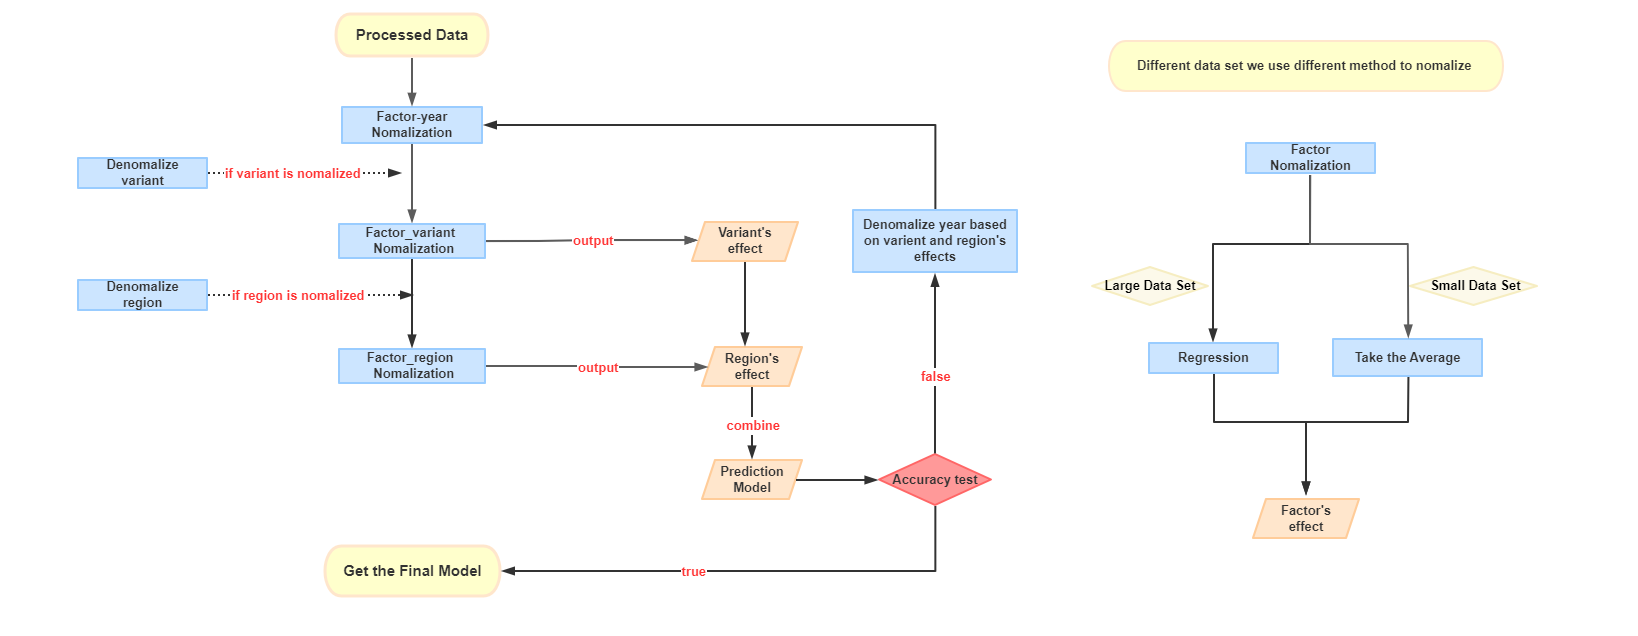
\includegraphics[width=1\textwidth]{Model1.png}
    \caption{Brief process of Model 1}\label{fig:Model1}
\end{figure}
A key aspect of Model 1's success is the heuristic approach employed during each normalization step. This method adapts to the size of the dataset, offering a more efficient and effective means of processing the data. For larger datasets, regression is performed, which capitalizes on the wealth of information available and can identify complex patterns and relationships. Conversely, for smaller datasets, the model calculates the average, providing a simpler and more straightforward representation of the data.

\begin{figure}[htbp]
    \centering
    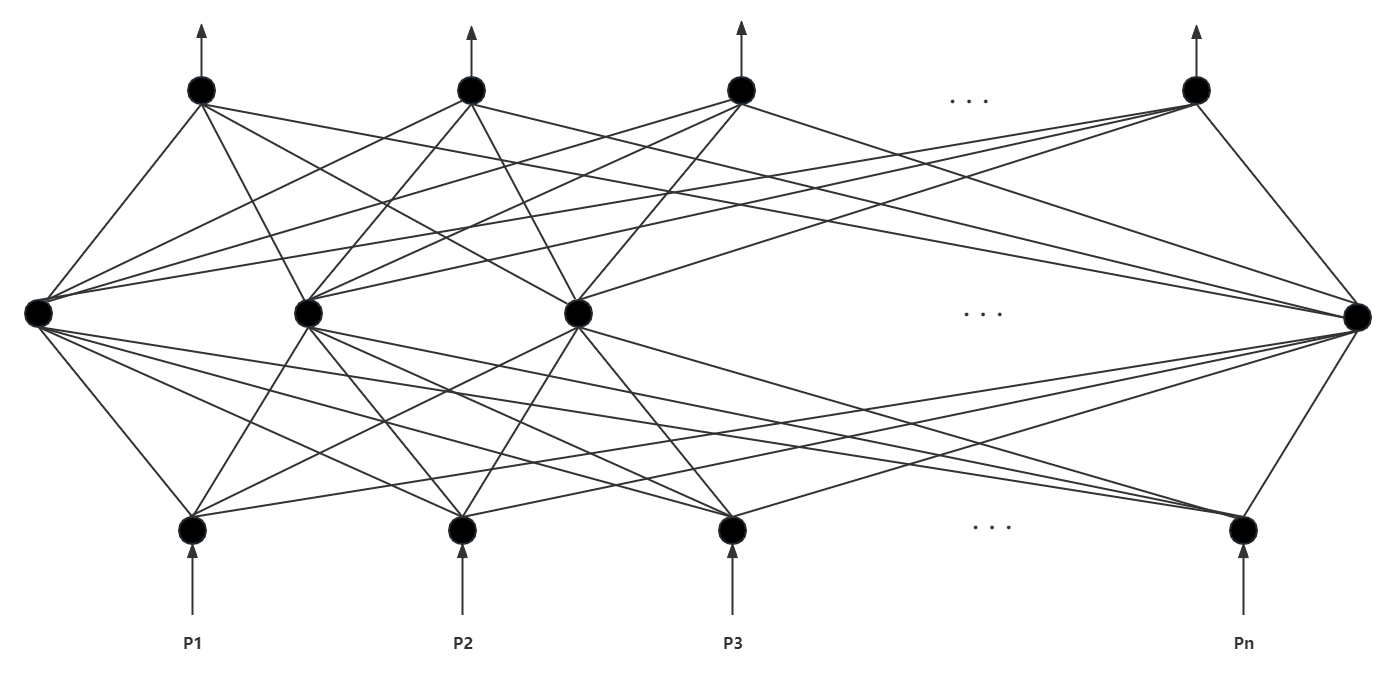
\includegraphics[width=.8\textwidth]{Hierarchical.png}
    \caption{Hierarchical Multiple Regression}\label{fig:Hierarchical}
\end{figure}

This adaptive heuristic approach has a significant impact on the accuracy of the model's predictions, as it tailors the normalization process to suit the specific characteristics of the dataset. By adjusting the method used based on dataset size, Model 1 is better able to understand the underlying patterns and relationships, leading to more accurate and reliable predictions.

Furthermore, the hierarchical structure of the model enables it to isolate the effects of individual variables, providing valuable insights into their specific contributions to the overall prediction. This granular understanding of the relationships between variables can be instrumental in guiding further analysis and informing decision-making processes.

In summary, Model 1 offers a powerful and adaptive approach to price prediction, harnessing the power of heuristic hierarchical multiple regression to deliver accurate and reliable results. By tailoring the normalization process to suit the characteristics of the dataset and iteratively refining the model's understanding of variable relationships, Model 1 provides a robust and versatile tool for predicting prices based on input variables such as Year, Region, and Variant.


\subsubsection{Model 2 \textemdash  Deep Forest Model}
However, \emph{Model 1} is somehow incomplete because \emph{Model 1} requires that the variant and region of the predicted data have appeared in the dataset before. 
However, in actual prediction, the variant and region may be opaque to the model. 
Taking the third question as an example, \emph{Model 1} can't predict the price of Hong Kong because the region effect of Hong Kong hasn't been evaluated by the model. 
Therefore, we use the \textbf{Deep Forest Model} to establish \emph{Model 2}.

\begin{figure}[htbp]
    \centering
    \includegraphics[width=1\textwidth]{Deep_forest1.png}
    \caption{Deep Forest Model}\label{fig:DF1}
\end{figure}

Deep forest is an ensemble learning model derived from the random forest approach. Ensemble learning techniques combine the predictions of multiple models to improve overall performance and reduce the risk of overfitting. In this case, the deep forest algorithm aggregates the results of numerous decision tree classifiers to produce a more accurate and stable prediction.


Unlike traditional decision trees, where each tree classifier is trained using the same dataset and strategy, deep forest introduces an element of randomness to increase the diversity of the model. By incorporating a randomized strategy for each tree classifier, the algorithm can capture a broader range of patterns and relationships within the data. This stochastic approach helps to minimize the correlation between individual trees, thereby improving the model's overall performance.

The deep forest model has several advantages over a single decision tree. First, it is more robust, as it leverages the wisdom of multiple tree classifiers to arrive at a consensus prediction. This aggregation process helps to reduce the impact of any single tree's errors, ensuring that the overall prediction is more reliable. Second, the deep forest model is less susceptible to overfitting, a common issue in machine learning where a model learns the training data too well and performs poorly on new, unseen data. By using a randomized strategy to train each tree classifier, deep forest reduces the likelihood of overfitting and improves the model's generalization capabilities.
\begin{figure}[htbp]
    \centering
    \includegraphics[width=1\textwidth]{Deep_forest2.png}
    \caption{Deep Forest Model}\label{fig:DF2}
\end{figure}
Another key benefit of the deep forest model is its ability to handle both categorical and continuous features, making it highly versatile for various types of problems. Additionally, the deep forest algorithm's structure enables it to be easily parallelized, allowing for efficient processing on multi-core processors or distributed computing environments.

In summary, the deep forest algorithm is an effective and robust machine learning method that addresses the limitations of traditional decision trees. By employing an ensemble learning approach and incorporating randomized strategies for training tree classifiers, deep forest models can deliver more accurate and reliable predictions. These features make the deep forest model particularly well-suited for challenging tasks, such as predicting prices, where a high degree of accuracy and stability is essential for success.

\begin{figure}[htbp]
    \centering
    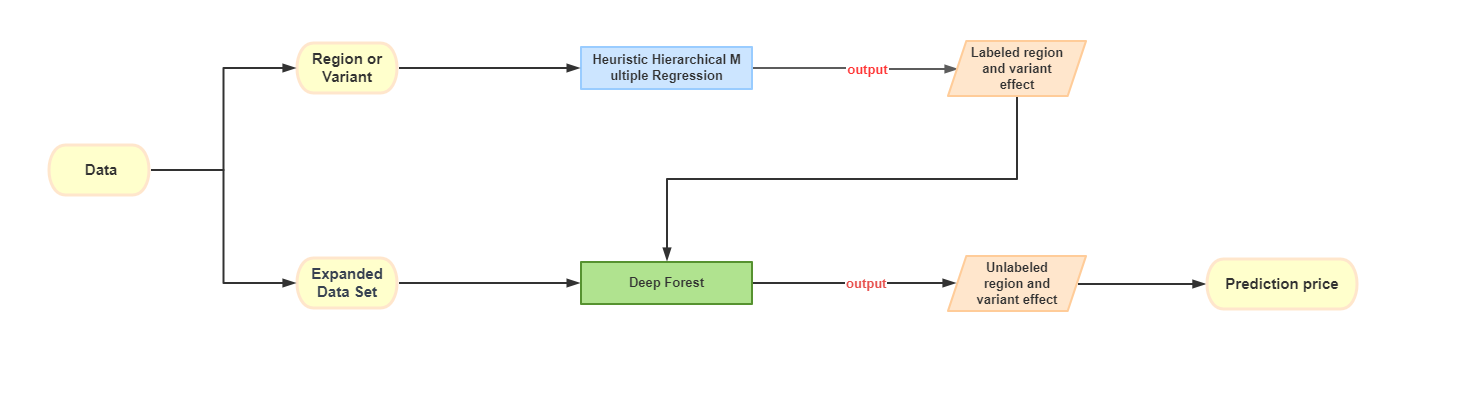
\includegraphics[width=1\textwidth]{Model2.png}
    \caption{Brief process of Model 2}\label{fig:Model2}
\end{figure}

As for \emph{Model 2}, we first expanded the dataset to obtain quantified data for regions and variants.
Specifically, for variants, we expanded data such as \texttt{draft}, \texttt{beam}, \texttt{water tank}, \texttt{fuel tank}, \texttt{cabins}, \texttt{displacement}, etc. 
For regions, we expanded data such as \texttt{GDP}, \texttt{Gini coefficient}, \texttt{Human Development Index}, etc. 
When dealing with unmarked variants and regions, we first used \emph{Model 1} to obtain the effects of marked variants and regions, and then applied the effects of marked variants and regions to the deep forest. 
By expanding the data for regression, we obtained the effects of unmarked variants and regions, and thus predicted the price.


\subsection{Model Accuracy Analysis}
Due to the limited data provided for some sailship types, 
they belong to imbalanced datasets. 
Therefore, we need to use as much data as possible for training to prevent the loss of small-sample data during training. 
Given that the leave-one-out method is not affected by random partition, 
it is effective for small-sample and imbalanced datasets, 
and can accurately evaluate the performance of the model, 
we used the \textbf{leave-one-out method} to analyze the model's error in the error analysis part.



For accuracy analysis, we use the correlation coefficient $R$ and Mean Absolute Percentage Error (MAPE) as evaluation metrics.
$$R(\textbf{X},\textbf{Y})=\frac{\text{cov}(\textbf{X},\textbf{Y})}{\sqrt{\text{var}[\textbf{X}] \text{v         ar}[\textbf{Y}]}}$$
$$\text{MAPE} = \frac{\sum_{i = 1}^n (\frac{|\textbf{P} - \textbf{Q}|}{\textbf{P}} \times 100\%)}{n}$$
where:
    $$\text{var}(\textbf{X})=\frac{\sum_{i=1}^{n}(\textbf{X}_i-\overline{\textbf{X}})(\textbf{X}_i-\overline{\textbf{X}})}{n-1}$$
    $$\text{cov}(\textbf{X},\textbf{Y})=\frac{\sum_{i=1}^{n}(\textbf{X}_i-\overline{\textbf{X}})(\textbf{Y}_i-\overline{\textbf{Y}})}{n-1}$$
\section{Regional Effect Analysis}
Applying \emph{Model 1}, we can easily abstract the effect of each region. 
Therefore, by normalizing the year and variant, 
we can clearly see the effect of each region(see Figure \ref{fig:region_effect}).

\begin{figure}[htbp]
    \centering
    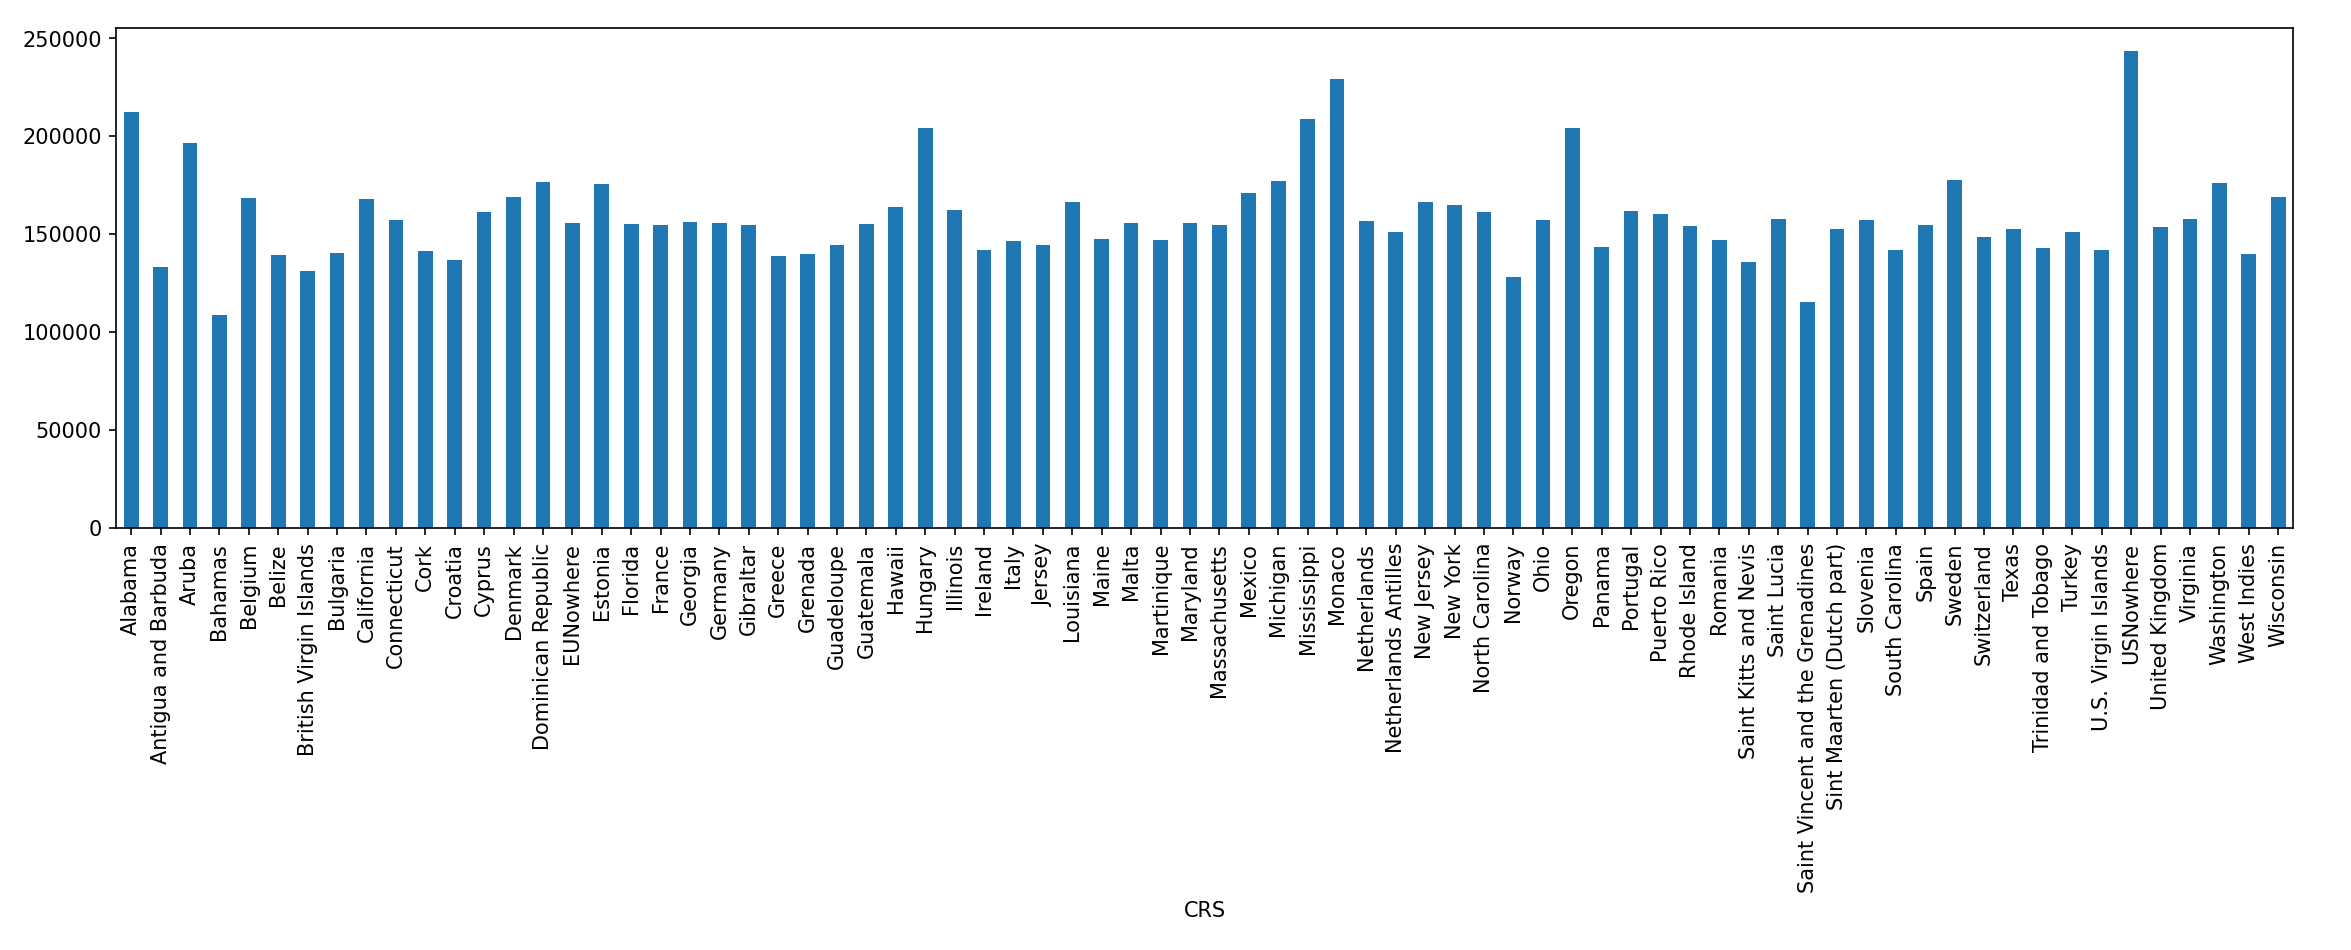
\includegraphics[width=1\textwidth]{region_effect.png}
    \caption{Region Effect}\label{fig:region_effect}
\end{figure}


\section{The applicability of The Prediction Model in Hong Kong}
When applying our model to the Hong Kong region, 
we first assume that we can obtain the Year, Variant, and Region parameters for the used sailboats. 
For the given geographic regions, we start by using \emph{Model 2} to determine the Region Effect, leveraging the area's GDP data.

If the predicted Variant is present in the training set, 
we can directly use \emph{Model 1} to estimate the pricing by incorporating the Region Effect, Variant Effect, and Year. 
However, if the predicted Variant is not in the training set, we first need to use \emph{Model 2} to obtain the Variant Effect by considering factors such as beam, draft, and displacement. 
Once the Variant Effect is determined, we can then employ \emph{Model 1} to make the final price prediction.

This two-step approach enables us to adapt our models to different regions like Hong Kong and successfully predict used sailboat prices. 
By utilizing both \emph{Model 1} and \emph{Model 2} in tandem, we can account for regional influences, specific variant characteristics, 
and the age of the sailboat to provide accurate and reliable pricing estimates.



\section{Extended Inferences or Conclusion}


\section{Further Improvements}

\section{Strengths and Weaknesses}
\subsection{Strengths}

\textbf{Comprehensiveness:}
After the basic data processing, we significantly expanded the dataset, including extending the Variant to Draft, Beam, Displacement, Water tank, Fuel tank, and Cabin, as well as expanding the Region to GDP, HDI, and Gini coefficient. We performed correlation tests for each variable, making the modeling process extensive and comprehensive.

\textbf{Innovative:}
Our model combines heuristic learning and hierarchical multivariate regression, obtaining accurate predictions through continuous iteration. This creative and highly applicable model is well-suited for the task at hand.Additionally, we used a deep forest algorithm to extend the prediction of unknown variants and regions, enhancing the model's versatility. 

\textbf{Accuracy:}
Our model performs exceptionally well in terms of both error analysis and accuracy, achieving 94.91\% on the Catamarans test set and 92.71\% on the Monohulled Boats test set. Moreover, the model can improve its accuracy through self-iteration and possesses heuristic learning capabilities.

\textbf{Applicability:}
When applied to the Hong Kong market, the model maintains a high level of accuracy, demonstrating its excellent applicability. 

\subsection{Weaknesses}
\textbf{Time consuming:}
The model can achieve satisfactory regression results after 2-3 iterations when processing the data for this task. However, when handling larger datasets, the increased number of iterations may result in additional time costs.

\textbf{Lack of geography  factor analysis:}
Due to the difficulty in obtaining geographical data and the challenge of analyzing and quantifying factors such as climate, the model does not include geographical factors. Despite this limitation, the model still provides valuable insights and accurate predictions for the used sailboat market.

\section{Conclusion}
In conclusion, our study has successfully addressed the challenges faced by brokers in the used sailboat market, where pricing is influenced by a myriad of factors such as brand, variant, age, depreciation rates, local consumption levels, and geographical environments. By developing a comprehensive and robust model that combines Heuristic Hierarchical Multiple Regression and Deep Forest Models, we have created a valuable tool that allows brokers and other stakeholders in the sailboat market to make well-informed decisions and ensure fair pricing practices.

Our meticulous data cleaning, expansion, and pre-analysis processes enabled us to establish a strong foundation for subsequent modeling efforts. Through Adaptive Density-Based Clustering and Linear interpolation techniques, we were able to identify patterns and trends in the data, providing crucial insights for our modeling approach.

The Heuristic Hierarchical Multiple Regression Model allowed us to establish the relationships between sailboat prices and factors such as year, region, and variant. Moreover, it enabled us to abstract the effect of regions and variants on sailboat prices, capturing the interactions between these variables and their influence on pricing.

By employing the Deep Forest Model, we trained the relationship between region and variant factors and their respective effects. This advanced ensemble learning technique enabled us to predict the effect of unknown regions and variants, which in turn allowed us to further predict their prices.

Our model has proven to be highly effective, achieving remarkable accuracy levels of 94.91\% on the Catamarans test set and 92.71\% on the Monohulled Boats test set. These results demonstrate the model's strong performance and applicability to real-world scenarios. Furthermore, the model's self-iteration and heuristic learning capabilities ensure that it can continuously improve its accuracy, making it an invaluable tool for brokers in the used sailboat market.

When applied to the Hong Kong market, our model maintained a high level of accuracy, showcasing its excellent applicability across different regions. The model's ability to achieve satisfactory regression results after 2-3 iterations is particularly noteworthy, as it demonstrates its efficiency and effectiveness in handling diverse datasets.

While our model does not currently include geographical factors due to the challenges in obtaining and quantifying geographical data, future research could explore incorporating these factors to further enhance the model's predictive capabilities.

In summary, our study has successfully developed a powerful and versatile model that can assist brokers in the used sailboat market in making more reasonable and comprehensive evaluations, ultimately leading to more rational and fair pricing practices. By combining the strengths of Heuristic Hierarchical Multiple Regression and Deep Forest Models, we have created a valuable tool that can be applied to various markets and datasets, making it an invaluable asset for brokers and stakeholders in the used sailboat market.
% 以下为信件/备忘录部分,不需要可自行去掉
% 如有需要可将整个 letter 环境移动到文章开头或中间
% 请在第二个花括号内填写标题,如「信件」(Letter)或「备忘录」(Memorandum)
\begin{letter}{Report}
\noindent\rule[0.25\baselineskip]{\textwidth}{2pt} 
\begin{flushleft}  % 左对齐环境,无首行缩进
\textbf{To:} Heishan Yan\\
\textbf{From:} Team 1234567\\
\textbf{Date:} October 1st, 2019\\
\textbf{Subject:} A better choice than MS Word: \LaTeX
\end{flushleft}

In the memo, we want to introduce you an alternate typesetting program to the prevailing MS Word: \textbf{\LaTeX}. In fact, the history of \LaTeX\ is even longer than that of MS Word. In 1970s, the famous computer scientist Donald Knuth first came out with a typesetting program, which named \TeX\ \ldots

Firstly, \ldots

Secondly, \ldots

Lastly, \ldots

According to all those mentioned above, it is really worth to have a try on \LaTeX! 

\noindent\rule[0.25\baselineskip]{\textwidth}{2pt} 
\end{letter}
\clearpage

% 参考文献,此处以 MLA 引用格式为例
\begin{thebibliography}{99}
\bibitem{1} Zhi-Hua Zhou, Ji Feng, Deep forest, \emph{National Science Review}, January 2019, from\url{https://doi.org/10.1093/nsr/nwy108}.
\bibitem{2} Eberly, L.E. (2007). Multiple Linear Regression. \emph{Methods in Molecular Biology}, from \url{https://doi.org/10.1007/978-1-59745-530-5_9}.
\bibitem{3} A. Ogunleye and Q. -G. Wang, "XGBoost Model for Chronic Kidney Disease Diagnosis," in \emph{IEEE/ACM Transactions on Computational Biology and Bioinformatics}.
\bibitem{4} Ingo Steinwart. "Fully adaptive density-based clustering." Ann. Statist, from \url{https://doi.org/10.1214/15-AOS1331}.
\bibitem{5} Reiss, K., Renkl, A. Learning to prove: The idea of heuristic examples. \emph{Zentralblatt für Didaktik der Mathematik}, from \url{https://doi.org/10.1007/BF02655690}.
\bibitem{6} Larson M G. Analysis of variance[J]. Circulation.
\bibitem{7} Witten I H, Frank E, Hall M A, et al. Practical machine learning tools and techniques[C].
\bibitem{8} Myles A J, Feudale R N, Liu Y, et al. An introduction to decision tree modeling[J].
\bibitem{9} Biau G, Scornet E. A random forest guided tour[J].
\bibitem{10} Genesove D. Adverse selection in the wholesale used car market[J].
\bibitem{11} Bernard H R, Ryan G. Text analysis[J]. 
\bibitem{12} Davis P J. Interpolation and approximation[M]. Courier Corporation, 1975.
\bibitem{13} Ganaie M A, Hu M, Malik A K, et al. Ensemble deep learning: A review[J].
\bibitem{14} Zhang M L, Zhou Z H. ML-KNN: A lazy learning approach to multi-label learning[J].
\bibitem{15} Madhulatha T S. An overview on clustering methods[J].
\bibitem{16} Limsombunchao V. House price prediction, hedonic price model.
\end{thebibliography}


% 以下为附录内容
% 如您的论文中不需要附录,请自行删除
\begin{subappendices}  % 附录环境

\section{Appendix A: Further on \LaTeX}
To clarify the importance of using \LaTeX\ in MCM or ICM, several points need to be covered, which are \ldots

To be more specific, \ldots

All in all, \ldots

Anyway, nobody \textbf{really} needs such appendix \ldots

\section{Appendix B: Program Codes}
Here are the program codes we used in our research.

% 代码环境示例三则
% 如您的论文不需要展示代码,请删除
% 更多用法,请参考 listings 宏包文档

% Python 代码示例
\begin{lstlisting}[language=Python, name={test.py}]
# Python code example
for i in range(10):
    print('Hello, world!')
\end{lstlisting}

% MATLAB 代码示例
\begin{lstlisting}[language=MATLAB, name={test.m}]
% MATLAB code example
for i = 1:10
    disp("hello, world!");
end
\end{lstlisting}

% C++ 代码示例
\begin{lstlisting}[language=C++, name={test.cpp}]
// C++ code example
#include <iostream>
using namespace std;

int main() {
    for (int i = 0; i < 10; i++)
        cout << "hello, world" << endl;
    return 0;
}
\end{lstlisting}

\end{subappendices}  % 附录内容结束

\end{document}  % 结束
